% IngredientIQ research paper, in the department paper format (single column, blue headings,
% literature survey table, grid tables with captions below, numbered references with DOIs).
% Build on Overleaf (upload the whole paper/ folder, compiler pdfLaTeX) or: latexmk -pdf main.tex
% Numbers, tables and figures are generated by scripts/make_paper_assets.py: never type a result by hand.
% House style: no em dashes anywhere (use commas, colons, semicolons or parentheses).
\documentclass[11pt,a4paper]{article}
\usepackage[a4paper,margin=2.5cm]{geometry}
\usepackage[T1]{fontenc}
\usepackage[sfdefault]{carlito}          % metric clone of Calibri, as in the template
\usepackage{amsmath,amssymb}
\usepackage{graphicx}
\usepackage[table]{xcolor}
\usepackage{array,longtable,tabularx}
\usepackage{xspace}
\usepackage{enumitem}
\usepackage{titlesec}
\usepackage[labelsep=colon,font={small,it},skip=6pt]{caption}
\usepackage{tikz}
\usetikzlibrary{arrows.meta,positioning}
\usepackage[colorlinks=true,urlcolor=linkblue,linkcolor=black,citecolor=black]{hyperref}
\usepackage{xurl}
\graphicspath{{figures/}}

\definecolor{headblue}{RGB}{46,116,181}   % heading colour of the template
\definecolor{headfill}{RGB}{217,226,243}  % table header shading
\definecolor{groupfill}{RGB}{242,242,242} % table group rows (e.g. "All, Rating")

% Let large tables and figures share a page with text instead of getting a page of their own
\renewcommand{\topfraction}{0.9}
\renewcommand{\bottomfraction}{0.8}
\renewcommand{\textfraction}{0.07}
\renewcommand{\floatpagefraction}{0.85}
\setcounter{totalnumber}{4}
\definecolor{linkblue}{RGB}{5,99,193}

\titleformat{\section}{\color{headblue}\LARGE\bfseries}{\thesection.}{0.4em}{}
\titleformat{\subsection}{\color{headblue}\Large\bfseries}{\thesubsection}{0.5em}{}
\titlespacing*{\section}{0pt}{16pt}{6pt}
\titlespacing*{\subsection}{0pt}{12pt}{4pt}
\setlength{\parindent}{0pt}
\setlength{\parskip}{6pt}
\setlist{itemsep=2pt,topsep=2pt}
\renewcommand{\arraystretch}{1.25}

% generated by scripts/make_paper_assets.py - do not edit
\newcommand{\NCatalogue}{8,494\xspace}
\newcommand{\NAnalysed}{5,547\xspace}
\newcommand{\NInScope}{6,320\xspace}
\newcommand{\NRating}{4,617\xspace}
\newcommand{\NRecRate}{1,529\xspace}
\newcommand{\NIngredientFeatures}{572\xspace}
\newcommand{\NCombinations}{134\xspace}
\newcommand{\NComparisons}{54\xspace}
\newcommand{\NBBetter}{0\xspace}
\newcommand{\NABetter}{21\xspace}
\newcommand{\NTests}{6,117\xspace}
\newcommand{\NSigRaw}{1,608\xspace}
\newcommand{\NSigAdj}{187\xspace}
\newcommand{\NRobust}{127\xspace}
\newcommand{\MaxLGBMGain}{0.040\xspace}
\newcommand{\MinIngredientShare}{43\xspace}
\newcommand{\MaxIngredientShare}{69\xspace}
\newcommand{\OnlyRatingRTwo}{0.08\xspace}
\newcommand{\ARatingRTwo}{0.24\xspace}
\newcommand{\OnlyLovesRTwo}{0.19\xspace}
\newcommand{\ALovesRTwo}{0.52\xspace}
\newcommand{\OnlyReviewsRTwo}{0.11\xspace}
\newcommand{\AReviewsRTwo}{0.44\xspace}
\newcommand{\OnlyHPAUC}{0.64\xspace}
\newcommand{\AHPAUC}{0.80\xspace}
\newcommand{\NAblationTests}{27\xspace}
\newcommand{\NAblationNominal}{7\xspace}
\newcommand{\NAblationFDR}{0\xspace}
\newcommand{\MinAblationQ}{0.13\xspace}
\newcommand{\NCategoryTests}{24\xspace}
\newcommand{\NCategoryNominal}{3\xspace}
\newcommand{\NCategoryFDR}{0\xspace}
\newcommand{\MinCategoryQ}{0.31\xspace}
\newcommand{\NSensitivityTests}{27\xspace}
\newcommand{\NSensitivityNominal}{0\xspace}
\newcommand{\NSensitivityFDR}{0\xspace}
\newcommand{\MinSensitivityQ}{0.41\xspace}


% Drafting marks. Colour groups (not \textcolor) so a mark may contain lists and paragraphs.
%   \todo{...}  red   only you can supply this
%   \draft{...} blue  AI-drafted text: rewrite in your own words, keep the facts, macros and citations
% Black prose was AI-drafted earlier, too. The final PDF must contain no red or blue text.
\newcommand{\todo}[1]{{\color{red}[TODO: #1]}}
\newcommand{\draft}[1]{{\color{blue!70!black}#1}}

\begin{document}

% ===================================================================== TITLE
\begin{center}
{\LARGE\bfseries Do Ingredients Predict Cosmetic Product Success?\\[2pt]
Brand Confounding and the Limits of Feature Attribution\par}
\vspace{8pt}
{\large Drishti Gupta, Arya Singh, Jhanvi Goel\par}
\vspace{2pt}
{\itshape Under the guidance of Ms.\ Anshika Negi, Assistant Professor, Department of IT\par}
\end{center}

% ===================================================================== ABSTRACT
\section*{Abstract}
\draft{Cosmetic products are increasingly marketed, and chosen, by their ingredients, yet whether ingredient composition is associated with commercial success beyond brand, category and price has rarely been tested. We study \NAnalysed{} deduplicated single-formula products from a public Sephora catalogue and four success indicators: rating, popularity, review count and recommendation rate. Every frequent ingredient and mined ingredient combination is tested for association with each indicator, both raw and with brand, subcategory and price held fixed. We then compare models trained on retail metadata alone (Model A) with the same models given \NIngredientFeatures{} additional ingredient features (Model B), under random and unseen-brand cross-validation with a corrected resampled $t$-test. Of \NSigRaw{} associations that are significant before adjustment, only \NRobust{} remain robust after it. Model B is significantly better than Model A in \NBBetter{} of \NComparisons{} comparisons, and this holds across ablations, product categories and data-construction choices. Yet SHAP assigns \MinIngredientShare{} to \MaxIngredientShare{}\% of the ingredient-aware model's attribution to ingredient features. Ingredient lists largely re-encode brand and category: they look important to a model without adding information. Claims that ingredients drive product success, and feature-attribution claims in general, therefore need explicit control for confounders.}

% ===================================================================== 1 INTRODUCTION
\section{Introduction}

\subsection{Background}
\draft{Ingredient lists have moved from the back of the package to the centre of beauty marketing. Products are sold on ``hero'' ingredients such as niacinamide, retinol or hyaluronic acid, and on the absence of others (``fragrance-free'', ``clean''). Consumers who prefer clean beauty products weigh sustainability, safety and ethicality when they choose~\cite{shim2024}, and recommender systems now estimate a product's efficacy directly from its ordered ingredient list~\cite{lee2024}. The implicit premise behind both is that what is in a formula shapes how well the product is received.

Whether that premise holds in market data is rarely tested. Online ratings and reviews are known to move sales~\cite{chevalier2006,babic2016,moen2017}, and product success can be predicted from listing attributes~\cite{aulya2025,sari2026}, but these studies report which attributes are predictive, not whether an attribute adds information that brand and price do not already carry. That distinction matters for ingredients in particular. Brands reuse ingredients, bases and preservative systems across their whole range, so an ingredient that a few popular brands favour will look ``successful'' even if it does nothing for the products that contain it. The same problem affects machine-learning models: a model given ingredients can use them as a stand-in for brand, and feature-attribution methods such as SHAP~\cite{lundberg2017shap} will then report the ingredients as important~\cite{kumar2020,molnar2022}.

We therefore ask two questions, each with an explicit control for brand. First, which ingredients and ingredient combinations are associated with success when brand, subcategory and price are held fixed? Second, do ingredient features improve the prediction of success beyond a model that already knows brand, category, price and existing popularity, including for brands the model has never seen?}

\subsection{Objectives}
\draft{\begin{itemize}
\item Build a reproducible, deduplicated ingredient--success dataset from the Sephora catalogue, with four success indicators and a composite high-performer label.
\item Test every frequent ingredient and mined ingredient combination for association with each indicator, both raw and adjusted for brand, subcategory and price, with correction for multiple testing.
\item Compare metadata-only models (Model A) with ingredient-augmented models (Model B) across three model families, under random and unseen-brand cross-validation, using a corrected significance test.
\item Measure how much SHAP attribution the ingredient-aware model gives to ingredient features, and cross-check the most important ones against the statistical tests.
\item Check that the conclusions survive ablation of feature families, analysis of further product categories and changes to data-construction choices.
\item Report all findings as associations in this dataset, without causal, medical or safety claims.
\end{itemize}}

% ===================================================================== 2 LITERATURE SURVEY
\section{Literature Survey}
\draft{The literature relevant to this study falls into four groups, matching the parts of our question: how online reviews and ratings relate to sales; how product success is predicted from product attributes; how cosmetic ingredients have been analysed computationally and how consumers perceive them; and the limits of feature attribution in machine learning. Table~\ref{tab:survey} summarises the fifteen sources; the subsections below discuss what they imply for our design.}

% colour group instead of \draft{...}: a longtable must not sit inside a macro argument
\begingroup\color{blue!70!black}\small
\begin{longtable}{|p{0.6cm}|p{3.0cm}|p{5.0cm}|p{6.1cm}|}
\hline
\rowcolor{headfill}\textbf{S.No.} & \textbf{Author(s) \& Year} & \textbf{Research Paper / Study Title} & \textbf{Key Findings} \\
\hline
\endfirsthead
\hline
\rowcolor{headfill}\textbf{S.No.} & \textbf{Author(s) \& Year} & \textbf{Research Paper / Study Title} & \textbf{Key Findings} \\
\hline
\endhead
1 & Chevalier \& Mayzlin (2006) & The Effect of Word of Mouth on Sales: Online Book Reviews & An improvement in a book's reviews raises its relative sales on that site; one-star reviews have a larger impact than five-star reviews; reviews are overwhelmingly positive. \\ \hline
2 & Babi\'{c} Rosario, Sotgiu, De Valck \& Bijmolt (2016) & The Effect of Electronic Word of Mouth on Sales: A Meta-Analytic Review of Platform, Product, and Metric Factors & Across 1,532 effect sizes from 96 studies, electronic word of mouth is positively correlated with sales (0.091), with the effect varying by platform, product and metric. \\ \hline
3 & Moen, Havro \& Bjering (2017) & Online Consumers Reviews: Examining the Moderating Effects of Product Type and Product Popularity on the Review Impact on Sales & On 1.1 million reviews of 4,600 products in 30 categories, reviews affect sales, most for subjectively evaluated and less popular products; ratings show signs of bias. \\ \hline
4 & Aulya \& Kusnawi (2025) & Evaluating Classification Models for Predicting Product Success in Indonesian E-Commerce & With success defined as sales above the median on 3,673 listings, Random Forest performed best (AUC 0.907); shop followers and price were the strongest predictors. \\ \hline
5 & Sari, Hartanto \& Fajri (2026) & Skincare Product Recommendation System Using Hybrid Ensemble Learning & A hybrid of content-based filtering, matrix factorisation on synthetic user data and a Random Forest meta-learner explained 83\% of the variance in ratings of over 7,500 skincare products. \\ \hline
6 & Lee, Yoon, Kim, Lee, Lee \& Yoo (2024) & Deep Learning-Based Skin Care Product Recommendation: A Focus on Cosmetic Ingredient Analysis and Facial Skin Conditions & A deep network reads a product's ordered ingredient list to estimate its efficacy and, combined with facial skin analysis, recommends personalised products. \\ \hline
7 & Wang et al. (2025) & Machine Learning-Based Screening of Cosmetic Ingredients Identifies Vat Blue 6 as a Thyroid Hormone Receptor $\beta$ Disruptor & A Random Forest model ranked cosmetic ingredients by predicted thyroid-receptor disruption; six of twelve top-ranked ingredients tested showed binding in the laboratory. \\ \hline
8 & Shim et al. (2024) & The Clean Beauty Trend Among Millennial and Generation Z Consumers & In a study of 120 consumers using 10 products, preference for clean beauty went with engaged shopping behaviour; its key attributes were sustainability, safety and ethicality. \\ \hline
9 & Rizqia \& Ichwani (2026) & Analisis Sentimen Ulasan Produk Skincare Sephora Menggunakan Algoritma BERT & Fine-tuned BERT classifies the sentiment of 4,683 social-media posts about Sephora skincare products into positive, neutral and negative. \\ \hline
10 & Lundberg \& Lee (2017) & A Unified Approach to Interpreting Model Predictions & Introduces SHAP, which attributes each prediction to features using Shapley values and unifies several earlier attribution methods. \\ \hline
11 & Kumar, Venkatasubramanian, Scheidegger \& Friedler (2020) & Problems with Shapley-Value-Based Explanations as Feature Importance Measures & Shapley-value importance has mathematical problems; fixing them requires further machinery such as causal reasoning, and it fits human-centred explanation goals poorly. \\ \hline
12 & Aas, Jullum \& L{\o}land (2021) & Explaining Individual Predictions When Features Are Dependent: More Accurate Approximations to Shapley Values & Kernel SHAP assumes independent features, which can mislead even for linear models; dependence-aware approximations are more accurate. \\ \hline
13 & Hooker, Mentch \& Zhou (2021) & Unrestricted Permutation Forces Extrapolation: Variable Importance Requires at Least One More Model & Permutation-based importance and dependence plots can be highly misleading when features are strongly dependent, because they force the model to extrapolate. \\ \hline
14 & Molnar et al. (2022) & General Pitfalls of Model-Agnostic Interpretation Methods for Machine Learning Models & Catalogues pitfalls of interpretation methods, including ignoring feature dependence and drawing unjustified causal conclusions. \\ \hline
15 & Geirhos et al. (2020) & Shortcut Learning in Deep Neural Networks & Models often learn shortcuts: decision rules that perform well on benchmarks but fail to transfer to harder, real-world conditions. \\ \hline
\caption{Literature survey summary.}
\label{tab:survey}
\end{longtable}
\endgroup

\subsection{Online Reviews, Ratings and Sales}
\draft{A long line of work links online reviews to sales. Chevalier and Mayzlin~\cite{chevalier2006} showed on Amazon and Barnes \& Noble that better reviews raise a book's relative sales, and that negative reviews weigh more than positive ones. A meta-analysis of 96 studies by Babi\'{c} Rosario et al.~\cite{babic2016} confirms a positive but modest average correlation between electronic word of mouth and sales, with large differences across platforms and products. Moen et al.~\cite{moen2017} find the effect strongest for subjectively evaluated and less popular products, and report signs of rating bias. Together these studies justify treating ratings, review counts and popularity as success indicators, while warning that they are noisy and shaped by factors other than product quality, which is why we restrict ratings to products with enough reviews and model each indicator separately.}

\subsection{Predicting Product Success from Product Attributes}
\draft{Product success can be predicted from listing attributes. Aulya and Kusnawi~\cite{aulya2025} compare seven classifiers on Indonesian marketplace listings and find tree ensembles best, with shop followers and price as the strongest predictors, that is, seller reputation and price rather than product content. Sari et al.~\cite{sari2026} predict skincare ratings well from brand, category and product attributes. Both studies report which attributes are predictive; neither asks whether a group of attributes adds information beyond the others. Our Model A versus Model B comparison asks exactly that, for ingredients.}

\subsection{Computational Analysis of Cosmetic Ingredients}
\draft{Ingredient lists have been used in three ways. Lee et al.~\cite{lee2024} estimate a product's efficacy from its ordered ingredient list and use it for personalised recommendation. Wang et al.~\cite{wang2025} screen cosmetic ingredients for a health risk with a Random Forest model and confirm several predictions in the laboratory. Consumer research shows that ingredient-related attributes such as safety matter to buyers of clean beauty products~\cite{shim2024}, and Sephora products have been studied through review sentiment~\cite{rizqia2026}. These works treat ingredients as content to recommend from, or as risks to screen for. None tests whether ingredients are associated with market success once brand is accounted for.}

\subsection{Limits of Feature Attribution}
\draft{SHAP~\cite{lundberg2017shap} is the most common way to report which features a model relies on, but attribution describes the model, not the world. Kumar et al.~\cite{kumar2020} argue that Shapley-value importance has basic problems as a measure of feature importance. When features are dependent, as ingredients and brands are, attributions can mislead~\cite{aas2021}, and permutation-based importance forces models to extrapolate~\cite{hooker2021}. Molnar et al.~\cite{molnar2022} list ignoring feature dependence and drawing causal conclusions among the most common pitfalls. More broadly, models readily learn shortcuts that work on the data at hand but do not reflect the mechanism of interest~\cite{geirhos2020}; an ingredient that proxies for brand is such a shortcut.}

\subsection{Research Gap}
\draft{The surveyed work establishes that reviews and ratings relate to sales, that product success can be predicted from attributes, and that ingredients can be analysed computationally. It does not test whether ingredient composition is associated with market success beyond brand, category and price, and the attribution literature warns that importance scores alone cannot answer that question. This study fills the gap with adjusted association tests, an incremental-prediction comparison under unseen-brand validation, and a direct comparison of SHAP attribution with measured added value.}

% ===================================================================== 3 METHODOLOGY
\section{Methodology}

\begin{figure}[htbp]
\centering
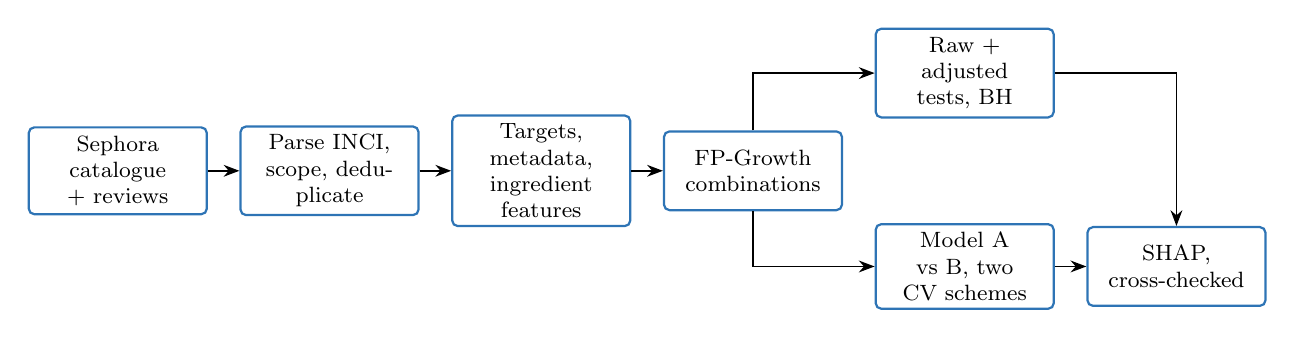
\begin{tikzpicture}[
  box/.style={draw=headblue, thick, rounded corners=2pt, align=center, font=\footnotesize, minimum height=1.0cm, text width=2.05cm, inner sep=3pt},
  arr/.style={-{Stealth[length=2mm]}, semithick}, node distance=0.4cm and 0.4cm]
\node[box] (raw) {Sephora catalogue\\+ reviews};
\node[box, right=of raw] (prep) {Parse INCI, scope, deduplicate};
\node[box, right=of prep] (feat) {Targets, metadata, ingredient features};
\node[box, right=of feat] (fp) {FP-Growth combinations};
\node[box, above right=0.15cm and 0.4cm of fp] (stats) {Raw + adjusted tests, BH};
\node[box, below right=0.15cm and 0.4cm of fp] (ml) {Model A vs B, two CV schemes};
\node[box, right=of ml] (shap) {SHAP, cross-checked};
\draw[arr] (raw) -- (prep); \draw[arr] (prep) -- (feat); \draw[arr] (feat) -- (fp);
\draw[arr] (fp) |- (stats); \draw[arr] (fp) |- (ml); \draw[arr] (ml) -- (shap);
\draw[arr] (stats.east) -| (shap.north);
\end{tikzpicture}
\caption{Analysis pipeline. All steps are deterministic and seeded; no language model is involved.}
\label{fig:pipeline}
\end{figure}

\subsection{Dataset}
We use the public Sephora product and review dataset~\cite{sephoradata}. The catalogue lists \NCatalogue{} products with brand, category hierarchy, price, average rating, review count, ``loves'' count and the raw ingredient (INCI) text. Ingredient strings were parsed into ordered ingredient entities, keeping nested parentheses and colour-index groups intact, and labelled by section: primary ingredients versus ``may contain'' shade lists. Fig.~\ref{fig:pipeline} summarises the analysis.

\subsection{Scope and Deduplication}
We analyse single-formula products that have an ingredient list, excluding multi-component kits, gift sets, minis and tools (Table~\ref{tab:dataset}). A mini and its full-size version share one formula; keeping both would place the same formula in training and test folds and inflate any ingredient model. We therefore merge products into families when they share a brand and either (a) the same name after removing size words or (b) an identical ingredient list, and keep the family member with the most reviews. This yields \NAnalysed{} products. Ingredient spellings are canonicalised (for example, \emph{aqua/water/eau} becomes \emph{water}), and only primary-section ingredients are used.

\subsection{Success Indicators}
We study four indicators and one composite:
\begin{itemize}
\item \emph{Rating}: the catalogue average rating, used only for products with at least 25 reviews (\NRating{} products), since ratings from a handful of reviews are dominated by noise.
\item \emph{Popularity}: $\log(1+\text{loves})$.
\item \emph{Engagement}: $\log(1+\text{reviews})$.
\item \emph{Recommendation rate}: the share of reviewers recommending the product, from at least 25 votes. Reviews are available for Skincare only, so this indicator covers \NRecRate{} Skincare products.
\item \emph{High performer}: a binary label for the top quartile of a composite score. The composite averages within-category percentile ranks of a shrunken rating, log loves and log reviews; ranking within category keeps the label from simply encoding the category.
\end{itemize}
Rating and recommendation rate are nearly interchangeable (Spearman $\rho=0.94$), whereas rating and popularity are weakly negatively related ($\rho=-0.15$), so we model the indicators separately.

\subsection{Feature Sets}
\emph{Baseline features (Model A)} are what a retailer knows without reading the label: brand and the three category levels (one-hot encoded, with brands of fewer than 10 products pooled); log price; value-price, on-sale, limited-edition, new, online-only, out-of-stock and exclusive flags; and variant count. Existing popularity (log loves and log reviews) enters Model A only where it is not circular, namely for rating and recommendation rate. Loves and review count are near-duplicates of each other, and the composite label is built from both, so for those three targets popularity is left out.

\emph{Ingredient features (added in Model B)}, \NIngredientFeatures{} in total:
\begin{itemize}
\item presence of the 300 most frequent ingredients;
\item list prominence $1-r/n$ of the 100 most frequent, where $r$ is the zero-based rank among $n$ ingredients, a coarse proxy for concentration;
\item the number of ingredients;
\item the share of each product's ingredients in 37 functional groups (for example humectant, emollient or UV filter), from a curated ingredient--function table;
\item \NCombinations{} combination indicators (Section~\ref{sec:combos}).
\end{itemize}

\subsection{Ingredient Combination Mining}
\label{sec:combos}
Testing all ingredient pairs is infeasible and mostly uninformative. We mine frequent itemsets with FP-Growth~\cite{han2000fpgrowth} separately within each category, keeping itemsets of two or three ingredients with support of at least 5\% and lift of at least 1.5 (which discards pairs that co-occur only because both are ubiquitous), and at most 30 per category so that fragrance allergen clusters do not dominate. Mining does not use the targets, so it introduces no outcome leakage. Two combinations named in our project proposal before the analysis, glycerin + sodium hyaluronate and glycerin + hyaluronic acid, are always tested and reported as pre-specified hypotheses.

\subsection{Association Tests}
For every scope (all products, and each category with at least 300 products), target and binary feature present in at least 30 and absent in at least 30 products, we run two tests.

\emph{Raw tests.} For continuous targets we use the Mann--Whitney $U$ test~\cite{mann1947} with Cliff's $\delta$~\cite{cliff1993} as effect size; for the high-performer label, a $\chi^2$ test with Cram\'er's $V$. Functional-group shares, binned into none, low and high, use the Kruskal--Wallis test~\cite{kruskal1952} with $\varepsilon^2$.

\emph{Adjusted test.} We regress the standardised target on the feature with brand and subcategory fixed effects and log price as controls, so each coefficient compares otherwise comparable products of the same brand and subcategory at the same price. All coefficients are computed at once via the Frisch--Waugh--Lovell theorem~\cite{frisch1933,lovell1963}: the controls are partialled out of the target and of every feature once, which gives exact per-feature OLS estimates, standard errors and 95\% confidence intervals.

Within each scope and target, raw and adjusted $p$-values are corrected separately with the Benjamini--Hochberg procedure~\cite{benjamini1995}, giving $q$-values. An association is called \emph{robust} if raw and adjusted $q<0.05$ with the same sign.

\subsection{Predictive Modelling: Model A versus Model B}
For each target we train three model families twice, on baseline features (Model A) and on baseline plus ingredient features (Model B), on identical folds: ridge or logistic regression with the penalty chosen by inner cross-validation, so the wider Model B is not penalised by a fixed regularisation strength; Random Forest~\cite{breiman2001rf}; and LightGBM~\cite{ke2017lightgbm}. Classifiers are class-balanced. Primary metrics are $R^2$ and ROC-AUC; MAE, RMSE, accuracy, precision, recall and F1 are also reported.

We use two validation schemes. \emph{Random}: 5-fold cross-validation repeated three times (stratified for classification). \emph{Unseen brand}: five folds that each hold out whole brands, so the model cannot exploit knowing which brands are popular; this is where ingredient information should help most if it carries signal. Fold scores share training data, so a plain paired $t$-test is anti-conservative; we test the per-fold difference between B and A with the corrected resampled $t$-test of Nadeau and Bengio~\cite{nadeau2003}, which inflates the variance by $(1/k + n_{test}/n_{train})$. Models use scikit-learn~\cite{pedregosa2011sklearn}; tests use SciPy and statsmodels~\cite{seabold2010statsmodels}.

\subsection{Explainability}
We fit LightGBM Model B on all products of a scope and compute SHAP values~\cite{lundberg2017shap} with TreeExplainer. Global importance is the mean absolute SHAP value; direction is the sign of the correlation between a feature and its SHAP values. Importance is summed per feature family (metadata, ingredients, functional groups and combinations). Every ingredient feature in the top list is cross-checked against the adjusted tests and counts as \emph{confirmed} only if it is a robust association there with the same direction.

\subsection{Robustness Checks}
\draft{Three checks use LightGBM and correct for the number of comparisons within each check with Benjamini--Hochberg. \emph{Ablation} adds each ingredient feature family to Model A on its own, and also trains a model on ingredient features alone. \emph{Other categories} repeats the Model A versus Model B comparison within Makeup, Hair and Fragrance. \emph{Sensitivity} rebuilds the dataset with the review threshold set to 10 or 50 instead of 25, and without family deduplication.}

% ===================================================================== 4 RESULTS AND DISCUSSION
\section{Results and Discussion}

\subsection{Dataset Characteristics}
Table~\ref{tab:dataset} shows how the \NCatalogue{} catalogue products reduce to the \NAnalysed{} analysed products and how many products each success indicator covers.

\begin{table}[htbp]
\centering
\small
\begin{tabular}{|l|r|}
\hline
\rowcolor{headfill} \textbf{Stage / target} & \textbf{Products} \\
\hline
Catalogue products & 8,494 \\
\hline
\quad without an ingredient list & 950 \\
\hline
\quad multi-component kits & 713 \\
\hline
In scope (single formula; no sets, minis, tools) & 6,320 \\
\hline
\textbf{Analysed (one product per family)} & \textbf{5,547} \\
\hline
\hline
Rating ($\geq$25 reviews) & 4,617 \\
\hline
Loves, review count, high-performer label & 5,547 \\
\hline
Recommendation rate ($\geq$25 votes; Skincare only) & 1,529 \\
\hline
\hline
Ingredient features in Model B & 572 \\
\hline
\quad of which mined combinations & 134 \\
\hline
\end{tabular}
\caption{Dataset construction and target coverage.}
\label{tab:dataset}
\end{table}


\subsection{Most Raw Associations Are Brand and Category Effects}
Across \NTests{} feature tests, \NSigRaw{} are significant before adjustment ($q<0.05$). Only \NSigAdj{} remain significant once brand, subcategory and price are held fixed, and \NRobust{} pass both tests with the same sign (Fig.~\ref{fig:attrition}). The attrition is strongest in Fragrance: dozens of raw associations per target, of which at most one survives adjustment. Table~\ref{tab:robust} and Fig.~\ref{fig:assoc} list the largest robust associations; most are modest, about 0.2 to 0.5 outcome standard deviations.

\draft{The surviving associations are mostly not the actives that products are marketed on. For rating, the strongest negative associations are with vinylpyrrolidone film formers (VP/eicosene and VP/VA copolymers), typical of long-wear and styling formulas; the positive ones include a ferment filtrate used as a preservative and the conditioning agent behentrimonium chloride. For popularity, the volatile silicone cyclopentasiloxane, a texture agent, is the strongest positive association, while acetyl hexapeptide-8, a peptide marketed for anti-ageing, is among the strongest negative ones. A plausible reading is that texture and wear, which shoppers experience directly, leave more trace in ratings and popularity than claimed actives do. These associations can still reflect product types finer than our subcategories, and we do not interpret them causally.}

\begin{figure}[htbp]
\centering
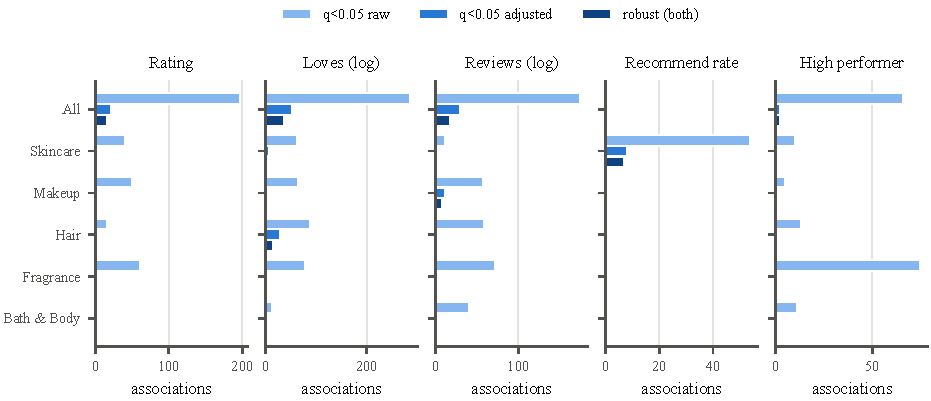
\includegraphics[width=\textwidth]{fig_attrition.pdf}
\caption{Number of ingredient and combination associations with $q<0.05$ before adjustment (raw), after adjusting for brand, subcategory and price, and in both tests with the same sign (robust).}
\label{fig:attrition}
\end{figure}

\begin{figure}[htbp]
\centering
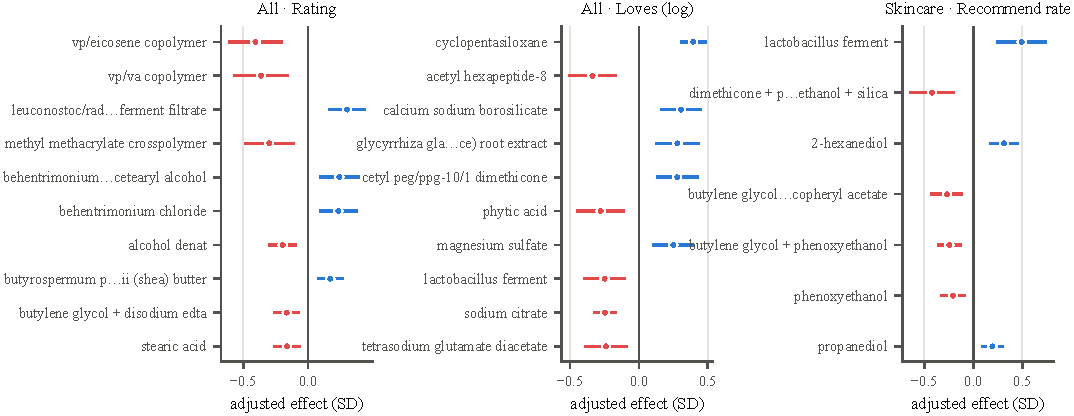
\includegraphics[width=\textwidth]{fig_associations.pdf}
\caption{Largest robust associations: brand-, subcategory- and price-adjusted effect in outcome standard deviations, with 95\% confidence intervals. Blue: positive; red: negative. Full names are in Table~\ref{tab:robust}.}
\label{fig:assoc}
\end{figure}

\begin{table}[htbp]
\centering
\footnotesize
\setlength{\tabcolsep}{3pt}
\begin{tabularx}{\linewidth}{|>{\raggedright\arraybackslash}X|l|r|r|r|c|r|}
\hline
\rowcolor{headfill} \textbf{Feature} & \textbf{Kind} & \textbf{$n$} & \textbf{Cliff's $\delta$} & \textbf{Adj.\ $\beta$} & \textbf{95\% CI} & \textbf{$q_{adj}$} \\
\hline
\multicolumn{7}{|l|}{\cellcolor{groupfill}\textbf{All, Rating}} \\
\hline
vp/eicosene copolymer & ingr. & 76 & $-0.471$ & $-0.407$ & [$-0.62$, $-0.19$] & 0.019 \\
\hline
vp/va copolymer & ingr. & 75 & $-0.291$ & $-0.364$ & [$-0.57$, $-0.15$] & 0.033 \\
\hline
leuconostoc/radish root ferment filtrate & ingr. & 211 & $+0.125$ & $+0.302$ & [$+0.16$, $+0.44$] & 0.005 \\
\hline
methyl methacrylate crosspolymer & ingr. & 91 & $-0.247$ & $-0.300$ & [$-0.49$, $-0.11$] & 0.048 \\
\hline
behentrimonium chloride + cetearyl alcohol & comb. & 163 & $+0.285$ & $+0.242$ & [$+0.09$, $+0.40$] & 0.048 \\
\hline
behentrimonium chloride & ingr. & 196 & $+0.258$ & $+0.234$ & [$+0.09$, $+0.38$] & 0.042 \\
\hline
\multicolumn{7}{|l|}{\cellcolor{groupfill}\textbf{All, Loves (log)}} \\
\hline
cyclopentasiloxane & ingr. & 301 & $+0.285$ & $+0.394$ & [$+0.30$, $+0.49$] & $<$0.001 \\
\hline
acetyl hexapeptide-8 & ingr. & 101 & $-0.222$ & $-0.337$ & [$-0.51$, $-0.16$] & 0.004 \\
\hline
calcium sodium borosilicate & ingr. & 116 & $+0.436$ & $+0.307$ & [$+0.16$, $+0.46$] & 0.003 \\
\hline
glycyrrhiza glabra (licorice) root extract & ingr. & 121 & $+0.277$ & $+0.280$ & [$+0.12$, $+0.44$] & 0.010 \\
\hline
cetyl peg/ppg-10/1 dimethicone & ingr. & 118 & $+0.467$ & $+0.279$ & [$+0.13$, $+0.43$] & 0.006 \\
\hline
phytic acid & ingr. & 88 & $-0.243$ & $-0.277$ & [$-0.45$, $-0.10$] & 0.022 \\
\hline
\multicolumn{7}{|l|}{\cellcolor{groupfill}\textbf{Skincare, Recommend rate}} \\
\hline
lactobacillus ferment & ingr. & 63 & $+0.207$ & $+0.493$ & [$+0.24$, $+0.75$] & 0.017 \\
\hline
dimethicone + phenoxyethanol + silica & comb. & 74 & $-0.189$ & $-0.424$ & [$-0.66$, $-0.19$] & 0.031 \\
\hline
2-hexanediol & ingr. & 290 & $+0.239$ & $+0.313$ & [$+0.17$, $+0.46$] & 0.009 \\
\hline
butylene glycol + phenoxyethanol + tocopheryl acetate & comb. & 175 & $-0.152$ & $-0.270$ & [$-0.43$, $-0.11$] & 0.049 \\
\hline
butylene glycol + phenoxyethanol & comb. & 455 & $-0.101$ & $-0.245$ & [$-0.37$, $-0.12$] & 0.015 \\
\hline
phenoxyethanol & ingr. & 813 & $-0.116$ & $-0.209$ & [$-0.33$, $-0.08$] & 0.049 \\
\hline
\end{tabularx}
\caption{Largest robust associations (raw and adjusted $q<0.05$, same sign).}
\label{tab:robust}
\end{table}


\subsection{Pre-specified Hypotheses}
Neither glycerin + sodium hyaluronate nor glycerin + hyaluronic acid is associated with rating (Table~\ref{tab:prespecified}). \draft{For popularity, glycerin + sodium hyaluronate shows a small negative adjusted association: among products of the same brand, subcategory and price, those containing the pair are slightly less loved. One reading is that the pair is so common in hydrating formulas that it does not set a product apart. We treat this as a lead rather than a finding, because the raw test misses significance after correction and the association disappears when deduplication is turned off (Section~\ref{sec:robustness}).} The niacinamide + zinc combination proposed in our project plan could not be tested, because zinc PCA is too rare in this catalogue.

\begin{table*}[t]
\centering
\caption{Pre-specified combinations from the project proposal.}
\label{tab:prespecified}
\footnotesize
\begin{tabular}{lllrrrrr}
\toprule
Combination & Scope & Target & $n$ & Raw & $p$ & Adj.\ $\beta$ & $p_{adj}$ \\
\midrule
glycerin + sodium hyaluronate & All & Rating & 733 & $-0.003$ & 0.912 & $-0.006$ & 0.875 \\
glycerin + hyaluronic acid & All & Rating & 91 & $+0.045$ & 0.459 & $+0.054$ & 0.589 \\
glycerin + sodium hyaluronate & All & Loves (log) & 884 & $-0.045$ & 0.033 & $-0.106$ & 0.001 \\
glycerin + hyaluronic acid & All & Loves (log) & 112 & $+0.049$ & 0.377 & $-0.118$ & 0.134 \\
glycerin + sodium hyaluronate & All & Reviews (log) & 884 & $+0.031$ & 0.143 & $-0.066$ & 0.056 \\
glycerin + hyaluronic acid & All & Reviews (log) & 112 & $+0.007$ & 0.895 & $-0.078$ & 0.351 \\
glycerin + sodium hyaluronate & All & Recommend rate & 475 & $-0.005$ & 0.866 & $-0.045$ & 0.428 \\
glycerin + hyaluronic acid & All & Recommend rate & 69 & $+0.099$ & 0.162 & $+0.096$ & 0.426 \\
glycerin + sodium hyaluronate & All & High performer & 884 & $+0.013$ & 0.431 & $+0.022$ & 0.578 \\
glycerin + hyaluronic acid & All & High performer & 112 & $+0.091$ & 0.037 & $+0.195$ & 0.036 \\
glycerin + sodium hyaluronate & Skincare & Rating & 484 & $-0.024$ & 0.440 & $-0.074$ & 0.179 \\
glycerin + hyaluronic acid & Skincare & Rating & 69 & $+0.055$ & 0.439 & $+0.065$ & 0.585 \\
glycerin + sodium hyaluronate & Skincare & Loves (log) & 589 & $-0.087$ & 0.003 & $-0.137$ & 0.002 \\
glycerin + hyaluronic acid & Skincare & Loves (log) & 87 & $+0.069$ & 0.279 & $-0.075$ & 0.430 \\
glycerin + sodium hyaluronate & Skincare & Reviews (log) & 589 & $-0.029$ & 0.317 & $-0.091$ & 0.054 \\
glycerin + hyaluronic acid & Skincare & Reviews (log) & 87 & $-0.025$ & 0.689 & $-0.071$ & 0.481 \\
glycerin + sodium hyaluronate & Skincare & Recommend rate & 475 & $-0.005$ & 0.866 & $-0.045$ & 0.428 \\
glycerin + hyaluronic acid & Skincare & Recommend rate & 69 & $+0.099$ & 0.162 & $+0.096$ & 0.426 \\
glycerin + sodium hyaluronate & Skincare & High performer & 589 & $+0.002$ & 0.977 & $-0.021$ & 0.674 \\
glycerin + hyaluronic acid & Skincare & High performer & 87 & $+0.148$ & 0.003 & $+0.336$ & 0.002 \\
\bottomrule
\end{tabular}
\par\smallskip
\parbox{\linewidth}{\scriptsize Raw: Cliff's $\delta$ (rate difference for high performer). Adj.\ $\beta$: brand-, subcategory- and price-adjusted difference in outcome SD. Unadjusted for multiple testing because the hypotheses were stated in advance.}
\end{table*}


\subsection{Ingredient Features Add No Significant Predictive Value}
Model B is significantly better than Model A in \NBBetter{} of \NComparisons{} comparisons and significantly worse in \NABetter{} (Fig.~\ref{fig:models}, Table~\ref{tab:models}). For LightGBM, the model best suited to many sparse features, the largest mean gain is \MaxLGBMGain{} and no gain is significant, under either random or unseen-brand validation. The significant losses come from the linear models and the Random Forest.

\draft{The losses have a technical explanation rather than meaning that ingredients are harmful. A ridge or logistic model applies one penalty to all columns, and no single strength suits both the few dense metadata features and the hundreds of sparse ingredient indicators, so tuning settles on a compromise that over-fits the indicators or under-uses the metadata. A Random Forest samples a fraction of the features at each split, so adding hundreds of weak columns lowers the chance that the strong brand and category features are available. LightGBM, which can ignore uninformative columns, neither gains nor loses significantly. This mirrors the finding of Aulya and Kusnawi~\cite{aulya2025} that seller reputation and price, not product content, drive predicted success.}

\begin{figure}[htbp]
\centering
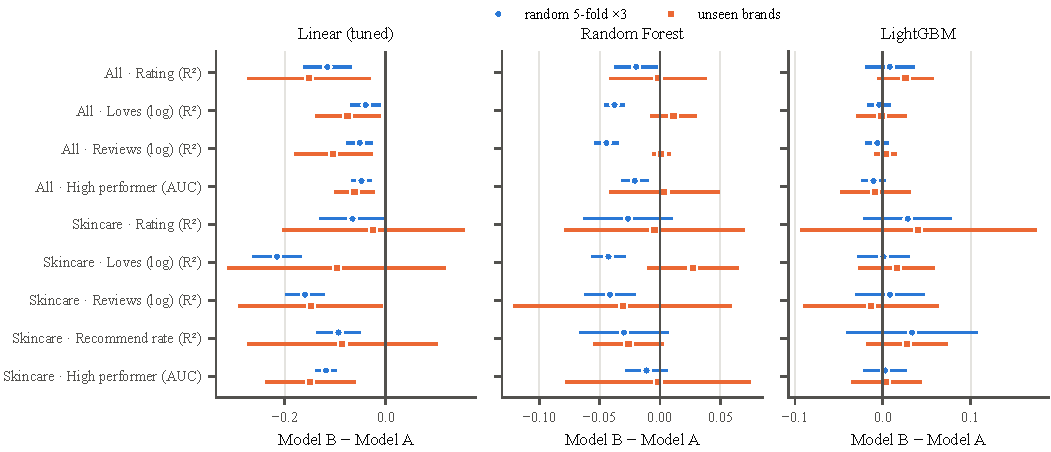
\includegraphics[width=\textwidth]{fig_model_comparison.pdf}
\caption{Model B minus Model A on the primary metric ($R^2$, or ROC-AUC for high performer): mean over folds with 95\% intervals from the corrected resampled variance. Intervals crossing zero indicate no significant difference.}
\label{fig:models}
\end{figure}

\begin{table}[htbp]
\centering
\small
\begin{tabular}{|l|l|l|l|r|r|r|r|r|c|}
\hline
\rowcolor{headfill} \textbf{Scope} & \textbf{Target} & \textbf{Split} & \textbf{Metric} & \textbf{A} & \textbf{B} & \textbf{$\Delta$} & \textbf{B wins} & \textbf{$p_{corr}$} & \textbf{Better} \\
\hline
All & Rating & random & $R^2$ & 0.242 & 0.250 & $+0.008$ & 10/15 & 0.540 & -- \\
\hline
All & Rating & unseen brand & $R^2$ & 0.115 & 0.141 & $+0.026$ & 4/5 & 0.085 & -- \\
\hline
All & Loves (log) & random & $R^2$ & 0.525 & 0.520 & $-0.004$ & 5/15 & 0.509 & -- \\
\hline
All & Loves (log) & unseen brand & $R^2$ & 0.346 & 0.345 & $-0.001$ & 3/5 & 0.901 & -- \\
\hline
All & Reviews (log) & random & $R^2$ & 0.438 & 0.432 & $-0.006$ & 5/15 & 0.339 & -- \\
\hline
All & Reviews (log) & unseen brand & $R^2$ & 0.276 & 0.280 & $+0.003$ & 3/5 & 0.505 & -- \\
\hline
All & High performer & random & AUC & 0.801 & 0.790 & $-0.011$ & 3/15 & 0.125 & -- \\
\hline
All & High performer & unseen brand & AUC & 0.745 & 0.736 & $-0.009$ & 1/5 & 0.582 & -- \\
\hline
\hline
Skincare & Rating & random & $R^2$ & 0.176 & 0.204 & $+0.028$ & 11/15 & 0.243 & -- \\
\hline
Skincare & Rating & unseen brand & $R^2$ & 0.025 & 0.065 & $+0.040$ & 4/5 & 0.451 & -- \\
\hline
Skincare & Loves (log) & random & $R^2$ & 0.441 & 0.441 & $+0.001$ & 8/15 & 0.950 & -- \\
\hline
Skincare & Loves (log) & unseen brand & $R^2$ & 0.169 & 0.185 & $+0.016$ & 3/5 & 0.362 & -- \\
\hline
Skincare & Reviews (log) & random & $R^2$ & 0.334 & 0.343 & $+0.008$ & 9/15 & 0.655 & -- \\
\hline
Skincare & Reviews (log) & unseen brand & $R^2$ & 0.150 & 0.137 & $-0.013$ & 2/5 & 0.655 & -- \\
\hline
Skincare & Recommend rate & random & $R^2$ & 0.199 & 0.233 & $+0.034$ & 11/15 & 0.348 & -- \\
\hline
Skincare & Recommend rate & unseen brand & $R^2$ & 0.124 & 0.151 & $+0.027$ & 4/5 & 0.176 & -- \\
\hline
Skincare & High performer & random & AUC & 0.773 & 0.776 & $+0.003$ & 10/15 & 0.804 & -- \\
\hline
Skincare & High performer & unseen brand & AUC & 0.705 & 0.709 & $+0.004$ & 3/5 & 0.794 & -- \\
\hline
\end{tabular}
\par\smallskip
\parbox{0.95\linewidth}{\footnotesize $p_{corr}$: Nadeau--Bengio corrected resampled $t$-test over folds (15 for random, 5 for unseen brand). Better: variant significantly better at 0.05.}
\caption{Model A (metadata) vs Model B (+ingredient features), LightGBM.}
\label{tab:models}
\end{table}


\subsection{Attribution Is Not Added Value}
Although adding ingredients does not improve prediction, the ingredient-aware model attributes \MinIngredientShare{} to \MaxIngredientShare{}\% of its mean absolute SHAP value to ingredient-derived features (Fig.~\ref{fig:shapgap}). Ingredient features partly encode brand and category, because brands reuse bases and preservative systems across their ranges, and a tree ensemble given both can split on either. Read in isolation, the SHAP summary would suggest that ingredients drive success; the controlled comparison shows that they add nothing beyond the metadata. \draft{This is the dependence problem described by Aas et al.~\cite{aas2021} and Hooker et al.~\cite{hooker2021}, observed in real data.}

\draft{Ingredients are not uninformative in themselves. A model given only ingredient features, with no metadata, reaches $R^2=\OnlyRatingRTwo$ for rating, \OnlyLovesRTwo{} for popularity and \OnlyReviewsRTwo{} for review count, and a ROC-AUC of \OnlyHPAUC{} for the high-performer label (Fig.~\ref{fig:ablation}), against \ARatingRTwo, \ALovesRTwo, \AReviewsRTwo{} and \AHPAUC{} for metadata alone. Ingredients therefore carry real information about success, but less than metadata, and, since adding them to metadata changes nothing, essentially the same information.}

\begin{figure}[htbp]
\centering
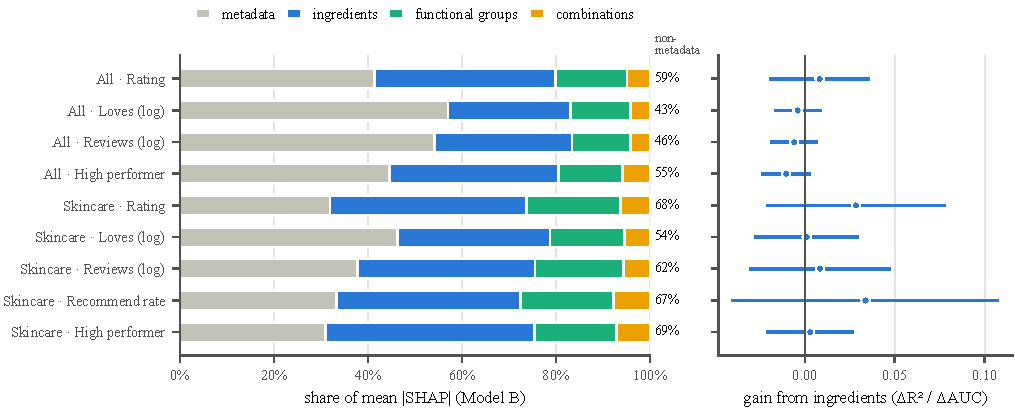
\includegraphics[width=\textwidth]{fig_shap_gap.pdf}
\caption{Left: share of mean absolute SHAP value by feature family in Model B (LightGBM); the percentage is the non-metadata share. Right: the actual gain in $R^2$ or ROC-AUC from adding those features (random CV, 95\% corrected intervals).}
\label{fig:shapgap}
\end{figure}

\subsection{Robustness}
\label{sec:robustness}
\emph{Ablation} (Table~\ref{tab:ablation}, Fig.~\ref{fig:ablation}). Of \NAblationTests{} comparisons that add a single ingredient feature family to Model A, \NAblationNominal{} have a nominal $p<0.05$ and none survives correction (smallest $q=\MinAblationQ$). The point estimates still differ by family: individual ingredients and combinations lean positive, most clearly for Skincare rating and recommendation rate, while functional-group shares lean negative and account for several of the nominally significant results.

\emph{Other categories} (Table~\ref{tab:categories}). Model B's largest gains appear in Fragrance, whose ingredient list is effectively its scent profile. \NCategoryNominal{} of \NCategoryTests{} comparisons have a nominal $p<0.05$; none survives correction (smallest $q=\MinCategoryQ$).

\emph{Sensitivity} (Table~\ref{tab:sensitivity}). With the review threshold at 10 or 50, or without family deduplication, no setting yields a significant gain: \NSensitivityNominal{} nominal and \NSensitivityFDR{} corrected out of \NSensitivityTests{} comparisons.

\draft{Taken together, the null result for the full ingredient feature set is robust to model choice, validation scheme, review threshold and deduplication. The point estimates nevertheless suggest where a better-powered study should look: individual ingredients in Skincare, and the ingredient list of fragrances, where it amounts to the scent profile.}

\begin{figure}[htbp]
\centering
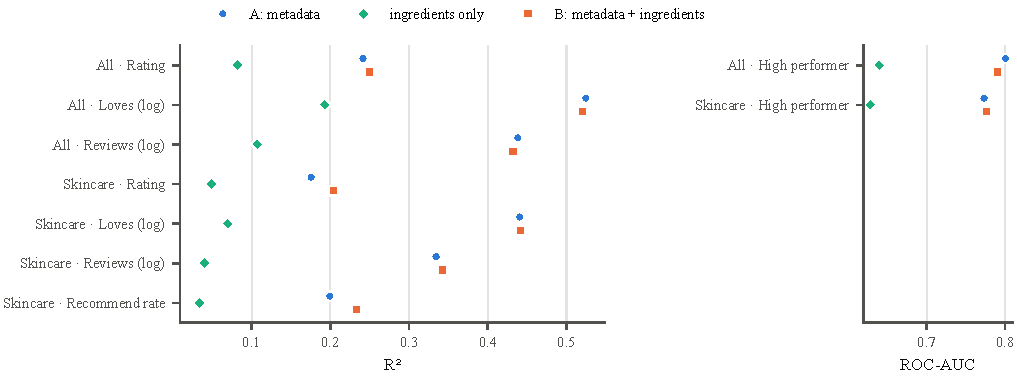
\includegraphics[width=\textwidth]{fig_ablation.pdf}
\caption{Model A, ingredients-only and Model B scores (LightGBM, random CV). Ingredients alone predict far less than metadata, and adding them to metadata changes little.}
\label{fig:ablation}
\end{figure}

\begin{table*}[t]
\centering
\caption{Ablation of ingredient feature families (LightGBM, random CV).}
\label{tab:ablation}
\footnotesize
\begin{tabular}{lllrrrr}
\toprule
Scope & Target & Variant & Score & $\Delta$ vs A & $p_{corr}$ & $q$ \\
\midrule
All & Rating & B & 0.250 & $+0.008$ & 0.540 & -- \\
All & Rating & A+ingredients & 0.252 & $+0.011$ & 0.410 & 0.692 \\
All & Rating & A+functional & 0.239 & $-0.003$ & 0.783 & 0.906 \\
All & Rating & A+combinations & 0.253 & $+0.011$ & 0.042 & 0.163 \\
All & Rating & ingredients\_only & 0.082 & $-0.159$ & $<$0.001 & -- \\
\midrule
All & Loves (log) & B & 0.520 & $-0.004$ & 0.509 & -- \\
All & Loves (log) & A+ingredients & 0.527 & $+0.002$ & 0.760 & 0.906 \\
All & Loves (log) & A+functional & 0.512 & $-0.012$ & 0.010 & 0.129 \\
All & Loves (log) & A+combinations & 0.530 & $+0.005$ & 0.323 & 0.623 \\
All & Loves (log) & ingredients\_only & 0.193 & $-0.331$ & $<$0.001 & -- \\
\midrule
All & Reviews (log) & B & 0.432 & $-0.006$ & 0.339 & -- \\
All & Reviews (log) & A+ingredients & 0.437 & $-0.001$ & 0.906 & 0.906 \\
All & Reviews (log) & A+functional & 0.422 & $-0.016$ & 0.005 & 0.129 \\
All & Reviews (log) & A+combinations & 0.441 & $+0.002$ & 0.515 & 0.732 \\
All & Reviews (log) & ingredients\_only & 0.107 & $-0.331$ & $<$0.001 & -- \\
\midrule
All & High performer & B & 0.790 & $-0.011$ & 0.125 & -- \\
All & High performer & A+ingredients & 0.793 & $-0.008$ & 0.288 & 0.598 \\
All & High performer & A+functional & 0.787 & $-0.014$ & 0.037 & 0.163 \\
All & High performer & A+combinations & 0.801 & $+0.000$ & 0.904 & 0.906 \\
All & High performer & ingredients\_only & 0.640 & $-0.161$ & $<$0.001 & -- \\
\midrule
Skincare & Rating & B & 0.204 & $+0.028$ & 0.243 & -- \\
Skincare & Rating & A+ingredients & 0.238 & $+0.062$ & 0.020 & 0.163 \\
Skincare & Rating & A+functional & 0.178 & $+0.002$ & 0.903 & 0.906 \\
Skincare & Rating & A+combinations & 0.216 & $+0.041$ & 0.058 & 0.189 \\
Skincare & Rating & ingredients\_only & 0.049 & $-0.127$ & 0.002 & -- \\
\midrule
Skincare & Loves (log) & B & 0.441 & $+0.001$ & 0.950 & -- \\
Skincare & Loves (log) & A+ingredients & 0.459 & $+0.019$ & 0.063 & 0.189 \\
Skincare & Loves (log) & A+functional & 0.419 & $-0.022$ & 0.125 & 0.306 \\
Skincare & Loves (log) & A+combinations & 0.448 & $+0.007$ & 0.515 & 0.732 \\
Skincare & Loves (log) & ingredients\_only & 0.070 & $-0.371$ & $<$0.001 & -- \\
\midrule
Skincare & Reviews (log) & B & 0.343 & $+0.008$ & 0.655 & -- \\
Skincare & Reviews (log) & A+ingredients & 0.350 & $+0.016$ & 0.366 & 0.659 \\
Skincare & Reviews (log) & A+functional & 0.313 & $-0.021$ & 0.141 & 0.318 \\
Skincare & Reviews (log) & A+combinations & 0.331 & $-0.003$ & 0.850 & 0.906 \\
Skincare & Reviews (log) & ingredients\_only & 0.040 & $-0.294$ & $<$0.001 & -- \\
\midrule
Skincare & Recommend rate & B & 0.233 & $+0.034$ & 0.348 & -- \\
Skincare & Recommend rate & A+ingredients & 0.255 & $+0.056$ & 0.101 & 0.272 \\
Skincare & Recommend rate & A+functional & 0.212 & $+0.013$ & 0.657 & 0.844 \\
Skincare & Recommend rate & A+combinations & 0.245 & $+0.046$ & 0.026 & 0.163 \\
Skincare & Recommend rate & ingredients\_only & 0.034 & $-0.166$ & 0.001 & -- \\
\midrule
Skincare & High performer & B & 0.776 & $+0.003$ & 0.804 & -- \\
Skincare & High performer & A+ingredients & 0.783 & $+0.010$ & 0.469 & 0.732 \\
Skincare & High performer & A+functional & 0.749 & $-0.025$ & 0.039 & 0.163 \\
Skincare & High performer & A+combinations & 0.770 & $-0.004$ & 0.636 & 0.844 \\
Skincare & High performer & ingredients\_only & 0.628 & $-0.145$ & $<$0.001 & -- \\
\bottomrule
\end{tabular}
\par\smallskip
\parbox{\linewidth}{\scriptsize Score: $R^2$, or ROC-AUC for high performer. $q$: Benjamini--Hochberg over the three single-family variants of all targets. B is the main comparison and ingredients\_only (no metadata) a reference point, so neither is tested here.}
\end{table*}

\begin{table*}[t]
\centering
\caption{Model A vs Model B within further categories (LightGBM).}
\label{tab:categories}
\footnotesize
\begin{tabular}{lllrrrrr}
\toprule
Scope & Target & Split & A & B & $\Delta$ & $p_{corr}$ & $q$ \\
\midrule
Makeup & Rating & random & 0.134 & 0.142 & $+0.009$ & 0.653 & 0.825 \\
Makeup & Rating & unseen brand & -0.015 & 0.047 & $+0.062$ & 0.057 & 0.313 \\
Makeup & Loves (log) & random & 0.334 & 0.332 & $-0.002$ & 0.914 & 0.954 \\
Makeup & Loves (log) & unseen brand & 0.167 & 0.185 & $+0.019$ & 0.466 & 0.822 \\
Makeup & Reviews (log) & random & 0.334 & 0.321 & $-0.012$ & 0.614 & 0.822 \\
Makeup & Reviews (log) & unseen brand & 0.168 & 0.184 & $+0.015$ & 0.295 & 0.770 \\
Makeup & High performer & random & 0.775 & 0.767 & $-0.008$ & 0.523 & 0.822 \\
Makeup & High performer & unseen brand & 0.716 & 0.733 & $+0.018$ & 0.701 & 0.842 \\
\midrule
Hair & Rating & random & 0.218 & 0.276 & $+0.058$ & 0.077 & 0.313 \\
Hair & Rating & unseen brand & 0.018 & 0.088 & $+0.070$ & 0.490 & 0.822 \\
Hair & Loves (log) & random & 0.478 & 0.479 & $+0.001$ & 0.957 & 0.957 \\
Hair & Loves (log) & unseen brand & 0.123 & 0.162 & $+0.039$ & 0.549 & 0.822 \\
Hair & Reviews (log) & random & 0.367 & 0.380 & $+0.012$ & 0.617 & 0.822 \\
Hair & Reviews (log) & unseen brand & 0.140 & 0.156 & $+0.016$ & 0.831 & 0.949 \\
Hair & High performer & random & 0.791 & 0.762 & $-0.029$ & 0.078 & 0.313 \\
Hair & High performer & unseen brand & 0.703 & 0.670 & $-0.033$ & 0.545 & 0.822 \\
\midrule
Fragrance & Rating & random & 0.113 & 0.217 & $+0.104$ & 0.047 & 0.313 \\
Fragrance & Rating & unseen brand & -0.002 & 0.066 & $+0.068$ & 0.566 & 0.822 \\
Fragrance & Loves (log) & random & 0.499 & 0.503 & $+0.005$ & 0.887 & 0.954 \\
Fragrance & Loves (log) & unseen brand & 0.210 & 0.329 & $+0.120$ & 0.046 & 0.313 \\
Fragrance & Reviews (log) & random & 0.441 & 0.471 & $+0.030$ & 0.239 & 0.718 \\
Fragrance & Reviews (log) & unseen brand & 0.281 & 0.339 & $+0.059$ & 0.321 & 0.770 \\
Fragrance & High performer & random & 0.809 & 0.842 & $+0.033$ & 0.029 & 0.313 \\
Fragrance & High performer & unseen brand & 0.766 & 0.808 & $+0.042$ & 0.220 & 0.718 \\
\bottomrule
\end{tabular}
\par\smallskip
\parbox{\linewidth}{\scriptsize $q$: Benjamini--Hochberg over all rows of this table.}
\end{table*}

\begin{table}[htbp]
\centering
\small
\begin{tabular}{|l|r|l|l|r|r|r|}
\hline
\rowcolor{headfill} \textbf{Setting} & \textbf{Products} & \textbf{Scope} & \textbf{Target} & \textbf{$\Delta$ (B--A)} & \textbf{$p_{corr}$} & \textbf{$q$} \\
\hline
reviews >= 10 & 5,547 & All & Rating & $-0.001$ & 0.921 & 0.921 \\
\hline
reviews >= 10 & 5,547 & All & Loves (log) & $-0.004$ & 0.726 & 0.921 \\
\hline
reviews >= 10 & 5,547 & All & Reviews (log) & $-0.004$ & 0.243 & 0.673 \\
\hline
reviews >= 10 & 5,547 & All & High performer & $-0.012$ & 0.091 & 0.573 \\
\hline
reviews >= 10 & 5,547 & Skincare & Rating & $+0.025$ & 0.127 & 0.573 \\
\hline
reviews >= 10 & 5,547 & Skincare & Loves (log) & $-0.003$ & 0.904 & 0.921 \\
\hline
reviews >= 10 & 5,547 & Skincare & Reviews (log) & $+0.010$ & 0.745 & 0.921 \\
\hline
reviews >= 10 & 5,547 & Skincare & Recommend rate & $+0.038$ & 0.299 & 0.673 \\
\hline
reviews >= 10 & 5,547 & Skincare & High performer & $-0.007$ & 0.744 & 0.921 \\
\hline
reviews >= 50 & 5,547 & All & Rating & $+0.007$ & 0.571 & 0.838 \\
\hline
reviews >= 50 & 5,547 & All & Loves (log) & $-0.004$ & 0.726 & 0.838 \\
\hline
reviews >= 50 & 5,547 & All & Reviews (log) & $-0.004$ & 0.243 & 0.700 \\
\hline
reviews >= 50 & 5,547 & All & High performer & $-0.012$ & 0.091 & 0.409 \\
\hline
reviews >= 50 & 5,547 & Skincare & Rating & $+0.095$ & 0.075 & 0.409 \\
\hline
reviews >= 50 & 5,547 & Skincare & Loves (log) & $-0.003$ & 0.904 & 0.904 \\
\hline
reviews >= 50 & 5,547 & Skincare & Reviews (log) & $+0.010$ & 0.745 & 0.838 \\
\hline
reviews >= 50 & 5,547 & Skincare & Recommend rate & $+0.047$ & 0.311 & 0.700 \\
\hline
reviews >= 50 & 5,547 & Skincare & High performer & $-0.007$ & 0.744 & 0.838 \\
\hline
no deduplication & 6,320 & All & Rating & $+0.024$ & 0.082 & 0.561 \\
\hline
no deduplication & 6,320 & All & Loves (log) & $-0.010$ & 0.230 & 0.561 \\
\hline
no deduplication & 6,320 & All & Reviews (log) & $-0.006$ & 0.593 & 0.725 \\
\hline
no deduplication & 6,320 & All & High performer & $+0.003$ & 0.673 & 0.725 \\
\hline
no deduplication & 6,320 & Skincare & Rating & $+0.057$ & 0.312 & 0.561 \\
\hline
no deduplication & 6,320 & Skincare & Loves (log) & $-0.033$ & 0.281 & 0.561 \\
\hline
no deduplication & 6,320 & Skincare & Reviews (log) & $+0.012$ & 0.466 & 0.698 \\
\hline
no deduplication & 6,320 & Skincare & Recommend rate & $+0.040$ & 0.232 & 0.561 \\
\hline
no deduplication & 6,320 & Skincare & High performer & $+0.006$ & 0.725 & 0.725 \\
\hline
\end{tabular}
\par\smallskip
\parbox{0.95\linewidth}{\footnotesize $q$: Benjamini--Hochberg within each setting.}
\caption{Sensitivity of the Model A vs B comparison (LightGBM, 5-fold).}
\label{tab:sensitivity}
\end{table}


\subsection{Discussion}
\draft{\emph{What the null result means.} In this catalogue, how well a product is rated, loved or reviewed is explained largely by who makes it, what kind of product it is and what it costs. Ingredient lists carry information about success, but almost none that brand, category and price do not already carry. This does not show that ingredients are irrelevant to how a product performs on the skin: our outcomes are market outcomes, and our ingredient features record presence and order, not dose. It does show that an ingredient list, read from the label, is a weak and largely redundant signal of market success.

\emph{Why ingredients still look important.} Brands have formulation habits: house bases, preservative systems, signature fragrances. An ingredient profile is therefore partly a fingerprint of the brand and the product type. A raw comparison picks up that fingerprint as an ``effect'', and a tree ensemble given both metadata and ingredients can split on either, so SHAP distributes credit between them; in the terms of Geirhos et al.~\cite{geirhos2020}, the ingredients act as a shortcut to brand. Attribution answers ``what did this model use?'', not ``what does this feature add?'' The gap between the two, \MinIngredientShare{} to \MaxIngredientShare{}\% of attribution with no significant gain, is in our view the most general lesson of the study.

\emph{Implications.} Claims that a given ingredient drives ratings or sales, whether made by brands, retailers or ingredient-checker tools, should be tested against comparable products of the same brand and type, not against the market average. More generally, feature-importance results from observational data should be accompanied by an incremental test, such as a with/without comparison or held-out groups, before features are described as drivers~\cite{molnar2022}.}

\subsection{Limitations}
\draft{\begin{itemize}
\item \emph{Observational, single-retailer, single-snapshot data.} Success is also shaped by marketing, shelf placement and brand history, which we do not observe; products that failed and were delisted are absent (survivorship bias).
\item \emph{Presence is not dose.} List position is only a coarse proxy for concentration, and ingredients below 1\% may be listed in any order.
\item \emph{Partial ingredient knowledge.} Functional-group shares rely on a curated table that maps only part of all ingredient occurrences.
\item \emph{Coverage.} Recommendation rate is available for Skincare only, and ratings cluster in a narrow, high range, which limits how much any model can explain.
\item \emph{Scope of claims.} All findings are associations in this dataset; none is a causal, medical or safety claim.
\end{itemize}}

% ===================================================================== 5 CONCLUSION
\section{Conclusion \& Future Scope}
\draft{We asked whether ingredient composition is associated with the market success of cosmetic products beyond brand, category and price. Most raw ingredient--success associations disappear once brand and subcategory are held fixed. Adding \NIngredientFeatures{} ingredient features to a metadata model yields no significant gain under random or unseen-brand validation, a result that holds across ablations, categories and data-construction choices. Ingredient features nonetheless receive a large share of SHAP attribution, because they largely re-encode brand and product type. Ingredient-based success claims, and feature-attribution claims in general, therefore need explicit control for confounders.

Several directions follow from what this study could not cover. Concentration data, rather than list position, would allow ingredient doses to be tested. Within-brand reformulations of the same product, where the brand stays fixed and the formula changes, would offer a cleaner natural experiment. Catalogues from other retailers would show whether the weak category-specific signals we observe, in Skincare and in Fragrance, generalise. Finally, dependence-aware attribution methods~\cite{aas2021} could be compared with plain SHAP on the same models to quantify how much of the attribution gap they close.}

% ===================================================================== 6 ACKNOWLEDGMENT
\section{Acknowledgment}
\draft{We thank Ms.\ Anshika Negi, Assistant Professor, Department of Information Technology, Bhagwan Parshuram Institute of Technology, for her guidance and supervision throughout this project. We are grateful to the creators of the publicly available Sephora product and review dataset~\cite{sephoradata}, and to the open-source communities behind scikit-learn, LightGBM, SHAP, SciPy, statsmodels, pandas and mlxtend, on which this work relies.}

\section*{Reproducibility}
Code, the analysis pipeline and all generated tables are available at \todo{repository URL}. Running \texttt{scripts/run\_research.py}, \texttt{scripts/run\_robustness.py} and \texttt{scripts/make\_paper\_assets.py} regenerates every number in this paper.

% References in the department format: numbered, [n] Initials Surname, "Title," Venue, vol., no., pp., year. DOI link.
% [1]-[15] are the literature survey (same numbers as Table 1); the rest are methods.
% Every entry was checked against Crossref or the publisher's page (October 2026), except [16].
% Before submitting, open each link once yourselves, and read the survey papers you discuss.
\begin{thebibliography}{99}
\setlength{\itemsep}{3pt}

\bibitem{chevalier2006}
J. A. Chevalier and D. Mayzlin, ``The Effect of Word of Mouth on Sales: Online Book Reviews,'' \emph{Journal of Marketing Research}, vol.~43, no.~3, pp.~345--354, 2006. \url{https://doi.org/10.1509/jmkr.43.3.345}

\bibitem{babic2016}
A. Babi\'{c} Rosario, F. Sotgiu, K. De Valck, and T. H. A. Bijmolt, ``The Effect of Electronic Word of Mouth on Sales: A Meta-Analytic Review of Platform, Product, and Metric Factors,'' \emph{Journal of Marketing Research}, vol.~53, no.~3, pp.~297--318, 2016. \url{https://doi.org/10.1509/jmr.14.0380}

\bibitem{moen2017}
{\O}. Moen, L. J. Havro, and E. Bjering, ``Online Consumers Reviews: Examining the Moderating Effects of Product Type and Product Popularity on the Review Impact on Sales,'' \emph{Cogent Business \& Management}, vol.~4, no.~1, p.~1368114, 2017. \url{https://doi.org/10.1080/23311975.2017.1368114}

\bibitem{aulya2025}
F. U. Aulya and K. Kusnawi, ``Evaluating Classification Models for Predicting Product Success in Indonesian E-Commerce,'' \emph{Jurnal Teknik Informatika (JUTIF)}, vol.~6, no.~4, pp.~2723--2739, 2025. \url{https://doi.org/10.52436/1.jutif.2025.6.4.5071}

\bibitem{sari2026}
Y. P. P. Sari, A. D. Hartanto, and I. N. Fajri, ``Skincare Product Recommendation System Using Hybrid Ensemble Learning,'' \emph{Journal of Applied Informatics and Computing}, vol.~10, no.~2, pp.~1587--1597, 2026. \url{https://doi.org/10.30871/jaic.v10i2.10461}

\bibitem{lee2024}
J. Lee, H. Yoon, S. Kim, C. Lee, J. Lee, and S. Yoo, ``Deep Learning-Based Skin Care Product Recommendation: A Focus on Cosmetic Ingredient Analysis and Facial Skin Conditions,'' \emph{Journal of Cosmetic Dermatology}, vol.~23, no.~6, pp.~2066--2077, 2024. \url{https://doi.org/10.1111/jocd.16218}

\bibitem{wang2025}
S. Wang, M. Nian, Y. Ma, X. Chen, X. Ji, C. Shi, X. Chen, and M. Fang, ``Machine Learning-Based Screening of Cosmetic Ingredients Identifies Vat Blue 6 as a Thyroid Hormone Receptor $\beta$ Disruptor,'' \emph{Environmental Science \& Technology}, vol.~59, no.~29, pp.~15005--15016, 2025. \url{https://doi.org/10.1021/acs.est.5c04327}

\bibitem{shim2024}
J. Shim, J. Woo, H. Yeo, S. Kang, B. Kwon, E. J. Lee, J. Oh, E. Jeong, J. Lim, and S. G. Park, ``The Clean Beauty Trend Among Millennial and Generation Z Consumers: Assessing the Safety, Ethicality, and Sustainability Attributes of Cosmetic Products,'' \emph{SAGE Open}, vol.~14, no.~2, 2024. \url{https://doi.org/10.1177/21582440241255430}

\bibitem{rizqia2026}
Y. N. Rizqia and A. Ichwani, ``Analisis Sentimen Ulasan Produk Skincare Sephora Menggunakan Algoritma BERT,'' \emph{Al-Kharaj: Jurnal Ekonomi, Keuangan \& Bisnis Syariah}, vol.~8, no.~9, pp.~4570--4581, 2026. \url{https://doi.org/10.47467/alkharaj.v8i9.13279}

\bibitem{lundberg2017shap}
S. M. Lundberg and S.-I. Lee, ``A Unified Approach to Interpreting Model Predictions,'' in \emph{Advances in Neural Information Processing Systems 30 (NeurIPS 2017)}, 2017. \url{https://arxiv.org/abs/1705.07874}

\bibitem{kumar2020}
I. E. Kumar, S. Venkatasubramanian, C. Scheidegger, and S. Friedler, ``Problems with Shapley-Value-Based Explanations as Feature Importance Measures,'' in \emph{Proceedings of the 37th International Conference on Machine Learning}, PMLR vol.~119, pp.~5491--5500, 2020. \url{https://proceedings.mlr.press/v119/kumar20e.html}

\bibitem{aas2021}
K. Aas, M. Jullum, and A. L{\o}land, ``Explaining Individual Predictions When Features Are Dependent: More Accurate Approximations to Shapley Values,'' \emph{Artificial Intelligence}, vol.~298, p.~103502, 2021. \url{https://doi.org/10.1016/j.artint.2021.103502}

\bibitem{hooker2021}
G. Hooker, L. Mentch, and S. Zhou, ``Unrestricted Permutation Forces Extrapolation: Variable Importance Requires at Least One More Model, or There Is No Free Variable Importance,'' \emph{Statistics and Computing}, vol.~31, no.~6, p.~82, 2021. \url{https://doi.org/10.1007/s11222-021-10057-z}

\bibitem{molnar2022}
C. Molnar, G. K\"{o}nig, J. Herbinger, T. Freiesleben, S. Dandl, C. A. Scholbeck, G. Casalicchio, M. Grosse-Wentrup, and B. Bischl, ``General Pitfalls of Model-Agnostic Interpretation Methods for Machine Learning Models,'' in \emph{xxAI: Beyond Explainable AI}, Lecture Notes in Computer Science, vol.~13200, pp.~39--68, 2022. \url{https://doi.org/10.1007/978-3-031-04083-2_4}

\bibitem{geirhos2020}
R. Geirhos, J.-H. Jacobsen, C. Michaelis, R. Zemel, W. Brendel, M. Bethge, and F. A. Wichmann, ``Shortcut Learning in Deep Neural Networks,'' \emph{Nature Machine Intelligence}, vol.~2, no.~11, pp.~665--673, 2020. \url{https://doi.org/10.1038/s42256-020-00257-z}

\bibitem{sephoradata}
\todo{Sephora Products and Skincare Reviews dataset: author/uploader, exact title, Kaggle URL, year and access date, copied from the Kaggle page you downloaded the data from.}

\bibitem{benjamini1995}
Y. Benjamini and Y. Hochberg, ``Controlling the False Discovery Rate: A Practical and Powerful Approach to Multiple Testing,'' \emph{Journal of the Royal Statistical Society: Series B (Methodological)}, vol.~57, no.~1, pp.~289--300, 1995. \url{https://doi.org/10.1111/j.2517-6161.1995.tb02031.x}

\bibitem{nadeau2003}
C. Nadeau and Y. Bengio, ``Inference for the Generalization Error,'' \emph{Machine Learning}, vol.~52, no.~3, pp.~239--281, 2003. \url{https://doi.org/10.1023/A:1024068626366}

\bibitem{han2000fpgrowth}
J. Han, J. Pei, and Y. Yin, ``Mining Frequent Patterns without Candidate Generation,'' in \emph{Proceedings of the 2000 ACM SIGMOD International Conference on Management of Data}, pp.~1--12, 2000. \url{https://doi.org/10.1145/342009.335372}

\bibitem{ke2017lightgbm}
G. Ke, Q. Meng, T. Finley, T. Wang, W. Chen, W. Ma, Q. Ye, and T.-Y. Liu, ``LightGBM: A Highly Efficient Gradient Boosting Decision Tree,'' in \emph{Advances in Neural Information Processing Systems 30 (NeurIPS 2017)}, 2017.

\bibitem{breiman2001rf}
L. Breiman, ``Random Forests,'' \emph{Machine Learning}, vol.~45, no.~1, pp.~5--32, 2001. \url{https://doi.org/10.1023/A:1010933404324}

\bibitem{cliff1993}
N. Cliff, ``Dominance Statistics: Ordinal Analyses to Answer Ordinal Questions,'' \emph{Psychological Bulletin}, vol.~114, no.~3, pp.~494--509, 1993. \url{https://doi.org/10.1037/0033-2909.114.3.494}

\bibitem{mann1947}
H. B. Mann and D. R. Whitney, ``On a Test of Whether One of Two Random Variables Is Stochastically Larger than the Other,'' \emph{The Annals of Mathematical Statistics}, vol.~18, no.~1, pp.~50--60, 1947. \url{https://doi.org/10.1214/aoms/1177730491}

\bibitem{kruskal1952}
W. H. Kruskal and W. A. Wallis, ``Use of Ranks in One-Criterion Variance Analysis,'' \emph{Journal of the American Statistical Association}, vol.~47, no.~260, pp.~583--621, 1952. \url{https://doi.org/10.1080/01621459.1952.10483441}

\bibitem{frisch1933}
R. Frisch and F. V. Waugh, ``Partial Time Regressions as Compared with Individual Trends,'' \emph{Econometrica}, vol.~1, no.~4, pp.~387--401, 1933. \url{https://doi.org/10.2307/1907330}

\bibitem{lovell1963}
M. C. Lovell, ``Seasonal Adjustment of Economic Time Series and Multiple Regression Analysis,'' \emph{Journal of the American Statistical Association}, vol.~58, no.~304, pp.~993--1010, 1963. \url{https://doi.org/10.1080/01621459.1963.10480682}

\bibitem{pedregosa2011sklearn}
F. Pedregosa \emph{et al.}, ``Scikit-learn: Machine Learning in Python,'' \emph{Journal of Machine Learning Research}, vol.~12, pp.~2825--2830, 2011. \url{https://jmlr.org/papers/v12/pedregosa11a.html}

\bibitem{seabold2010statsmodels}
S. Seabold and J. Perktold, ``Statsmodels: Econometric and Statistical Modeling with Python,'' in \emph{Proceedings of the 9th Python in Science Conference}, pp.~92--96, 2010. \url{https://doi.org/10.25080/Majora-92bf1922-011}

\end{thebibliography}


\end{document}
